\documentclass[t]{beamer}
\usetheme[deutsch]{KIT}
\setbeamercovered{transparent}
\setbeamertemplate{navigation symbols}{}

\KITfoot{Tutoriumsmaterial von Alexander Kwiatkowski, Michael Vollmer und Matthias Holoch \hspace{2.5cm} Basierend auf den Folien von Simon Stroh und Moritz v. Looz}
\usepackage[utf8]{inputenc}
\usepackage{amsmath}
\usepackage{ifthen}
\usepackage{amssymb}
\usepackage{tikz}
\usepackage{ngerman}
\usepackage[normalem]{ulem}
\usetikzlibrary{automata}
\usenavigationsymbols


\title{Theoretische Grundlagen der Informatik}
\subtitle{Tutorium}
\author{Alexander Kwiatkowski, Michael Vollmer und Matthias Holoch}

\institute[IKS]{Institut für Kryptographie und Sicherheit}

\TitleImage[height=\titleimageht]{images/tmaschine.png}

\newcommand{\N}{\ensuremath{\mathbb{N}}}
\newcommand{\M}{\ensuremath{\mathcal{M}}}
\newcommand{\classP}{\ensuremath{\mathcal{P}}}
\newcommand{\classNP}{\ensuremath{\mathcal{NP}}}
\newcommand{\co}{\ensuremath{\mathsf{co\text{-}}}}
\newcommand{\pot}{\ensuremath{\mathcal{P}}}
\newcommand{\abs}[1]{\ensuremath{\left\vert #1 \right\vert}}
\newcommand{\menge}[2]{\ensuremath{\left\lbrace #1 \,\middle\vert\, #2 \right\rbrace}}
\newcommand{\ducttape}[1]{\vspace{#1}}
\newcommand{\neglit}[1]{\overline{#1\vphantom{x^a}}}
\newcommand{\recipe}{\raisebox{-.3cm}{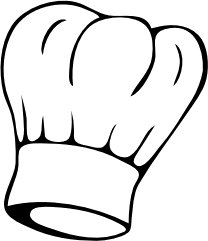
\includegraphics[scale=.15]{images/chefs-cap.png}}\hspace{0.2cm}}
\newcommand{\opt}[1]{\ensuremath{\text{OPT}(#1)}}
\newcommand{\A}[1]{\ensuremath{\mathcal{A}(#1)}}
\renewcommand{\O}[1]{\ensuremath{\mathcal{O}(#1)}}
\newcommand{\msout}[1]{\text{\sout{\ensuremath{#1}}}}

\newcommand{\invincible}{\setbeamercovered{invisible}} %  "Yesss! I am invincible!!" (Boris Grishenko)
\newcommand{\vincible}{\setbeamercovered{transparent}}
\renewcommand{\solution}[1]{\invincible \pause #1 \vincible}
\newcommand{\micropause}{\\[8pt]}

% \@ifundefined{tikzset}{}{\tikzset{initial text=}} % Text "start" bei Startknoten unterdrücken
\tikzstyle{every node}=[thick]
\tikzstyle{every line}=[thick]

\newcommand{\tutnr}[1]{
  \subtitle{Tutorium #1}
	\begin{frame}
		\maketitle
	\end{frame}
}

\newcommand{\uebnr}[1]{
  \subtitle{Anmerkungen zum #1. Übungsblatt}
	\begin{frame}
		\maketitle
	\end{frame}
}

\begin{document}

\newcommand{\start}[3]
{
  \draw (#1*2,#2*2) node{$#3$};
  \draw (#1*2,#2*2) circle(0.4cm);
  \draw [->] (#1*2-0.9,#2) -- (#1*2-0.4,#2);
}
\newcommand{\final}[3]
{
  \draw (#1*2,#2*2) node{$#3$};
  \draw (#1*2,#2*2) circle(0.4cm);
  \draw (#1*2,#2*2) circle(0.32cm);
}
\newcommand{\startfinal}[3]
{
  \draw (#1*2,#2*2) node{$#3$};
  \draw (#1*2,#2*2) circle(0.4cm);
  \draw (#1*2,#2*2) circle(0.32cm);
  \draw [->] (#1*2-0.9,#2) -- (#1*2-0.4,#2);
}
\newcommand{\state}[3]
{
  \draw (#1*2,#2*2) node{$#3$};
  \draw (#1*2,#2*2) circle(0.4cm);
}
\newcommand{\tol}[4]
{
  \draw (#1+#3,#2*2) node[above]{$#4$};
  \draw [->] (#1*2-0.4,#2*2) -- (#3*2+0.4,#2*2);
}
\newcommand{\tor}[4]
{
  \draw (#1+#3,#2*2) node[above]{$#4$};
  \draw [->] (#1*2+0.4,#2*2) -- (#3*2-0.4,#2*2);
}
\newcommand{\tot}[4]
{
  \draw (#1*2,#2+#3) node[right]{$#4$};
  \draw [->] (#1*2,#2*2+0.4) -- (#1*2,#3*2-0.4);
}
\newcommand{\tob}[4]
{
  \draw (#1*2,#2+#3) node[right]{$#4$};
  \draw [->] (#1*2,#2*2-0.4) -- (#1*2,#3*2+0.4);
}
\newcommand{\totl}[5]
{
  \draw (#1+#3,#2+#4) node[above right]{$#5$};
  \draw [->] (#1*2-0.283,#2*2+0.283) -- (#3*2+0.283,#4*2-0.283);
}
\newcommand{\totr}[5]
{
  \draw (#1+#3,#2+#4) node[above left]{$#5$};
  \draw [->] (#1*2+0.283,#2*2+0.283) -- (#3*2-0.283,#4*2-0.283);
}
\newcommand{\tobl}[5]
{
  \draw (#1+#3,#2+#4) node[below right]{$#5$};
  \draw [->] (#1*2-0.283,#2*2-0.283) -- (#3*2+0.283,#4*2+0.283);
}
\newcommand{\tobr}[5]
{
  \draw (#1+#3,#2+#4) node[below left]{$#5$};
  \draw [->] (#1*2+0.283,#2*2-0.283) -- (#3*2-0.283,#4*2+0.283);
}
\newcommand{\rloopl}[3]
{
  \draw (#1*2-1,#2*2) node[left]{$#3$};
  \draw [->] (#1*2-0.35,#2*2-0.2) arc (-30:-320:0.32cm);
}
\newcommand{\rloopr}[3]
{
  \draw (#1*2+1,#2*2) node[right]{$#3$};
  \draw [->] (#1*2+0.35,#2*2+0.2) arc (150:-140:0.32cm);
}
\newcommand{\rloopt}[3]
{
  \draw (#1*2,#2*2+1) node[above]{$#3$};
  \draw [->] (#1*2-0.2,#2*2+0.35) arc (240:-50:0.32cm);
}
\newcommand{\rloopb}[3]
{
  \draw (#1*2,#2*2-1) node[below]{$#3$};
  \draw [->] (#1*2+0.2,#2*2-0.35) arc (60:-230:0.32cm);
}
\newcommand{\lloopl}[3]
{
  \draw (#1*2-1,#2*2) node[left]{$#3$};
  \draw [->] (#1*2-0.35,#2*2+0.2) arc (30:320:0.32cm);
}
\newcommand{\lloopr}[3]
{
  \draw (#1*2+1,#2*2) node[right]{$#3$};
  \draw [->] (#1*2+0.35,#2*2-0.2) arc (-150:140:0.32cm);
}
\newcommand{\lloopt}[3]
{
  \draw (#1*2,#2*2+1) node[above]{$#3$};
  \draw [->] (#1*2+0.2,#2*2+0.35) arc (-60:230:0.32cm);
}
\newcommand{\lloopb}[3]
{
  \draw (#1*2,#2*2-1) node[below]{$#3$};
  \draw [->] (#1*2-0.2,#2*2-0.35) arc (-240:50:0.32cm);
}
\include{amsmath}

\tutnr{9}

\section{Komplexitätsklassen}
\subsection{Wiederholung: $\mathcal{P}, \mathcal{NP}$}
\begin{frame}
	\frametitle{$\mathcal{P}, \mathcal{NP}$}
	
	$\mathcal{P}$ ist die Klasse aller Sprachen, die von einer deterministischen Turingmaschine in Polynomialzeit erkannt werden.
	\begin{block}{Formal}
		$\mathcal{P} = \underset{k}{\cup}$ $TIME(n^k)$
	\end{block}
	
	$\mathcal{NP}$ ist die Klasse aller Sprachen, die von einer \textbf{nicht}deterministischen Turingmaschine in Polynomialzeit erkannt werden.
	\begin{block}{Formal}
		$\mathcal{NP} = \underset{k}{\cup}$ $NTIME(n^k)$
	\end{block}
\end{frame}

\subsection{$\mathcal{NP}$-schwer, $\mathcal{NP}$-vollständig}
\begin{frame}
	\frametitle{$\mathcal{NP}$-schwer, $\mathcal{NP}$-vollständig}
	Ein Problem liegt in \textbf{$\mathcal{NP}$-schwer} (Englisch: $\mathcal{NP}$-hard) falls es \textbf{mindestens} so schwer ist wie jedes Problem in $\mathcal{NP}$.
	
	Also: Ist $L \in \mathcal{NP}$-schwer, dann ist jedes $L' \in \mathcal{NP}$ polynomiell reduzierbar auf $L$.
	
	\begin{block}{Formal}
		$L \in \mathcal{NP}$-schwer $\Leftrightarrow \forall L' \in \mathcal{NP}: L' \preceq_p L$
	\end{block}
	
	Nach dieser Definition kann $L$ also auch schwerer sein als alle Probleme in $\mathcal{NP}$. Liegt $L$ zusätzlich auch noch selbst in $\mathcal{NP}$, so nennt man $L$ \textbf{$\mathcal{NP}$-vollständig}. (Englisch: $\mathcal{NP}$-complete)
\end{frame}

\subsection{Aufgabe B9 A3}
\begin{frame}
	\frametitle{Aufgabe B9 A3}
	Beweisen Sie folgende Aussagen:
	\begin{enumerate}
	\item Die Klasse $\mathcal{NP}$ ist unter Schnittbildung abgeschlossen.
	\item Die Klasse $\mathcal{NP}$ ist unter Vereinigung abgeschlossen.
	\end{enumerate}
	Dabei nehmen wir an, dass alle Sprachen "uber dem bin"aren Alphabet $\Sigma =
	\{0,1\}$ definiert sind.
\end{frame}

\section{CLIQUE}
\begin{frame}
	\frametitle{CLIQUE}
	\begin{block}{Kurzdefinition}
	Enthält der Graph eine Teilgraph von mindestens n Knoten, bei der jeder Knoten eine Kante zu jedem anderen Knoten des Teilgraphs hat?
	\end{block}
	\begin{block}{Formal}
	Gegeben: Ein ungerichteter Graph $G = (V,E)$ mit Knoten $v \in V$ und Kanten $e=(v_1, v_2)\in E$ mit $v_1, v_2 \in V$ und und eine $n \in \mathbb{N}$.\\
	Gesucht: Ein Teilgraph $G' = (V',E')$ mit $|V'|\ge n$ und $\forall v'_1, v'_2\in V':\exists e'\in E': e'=(v_1,v_2)$.
	\end{block}
\end{frame}
\begin{frame}
	\frametitle{Beispiel}
	\textbf{Gibt es eine Clique der Größe 4 in diesem Graphen?}
	\begin{center}
	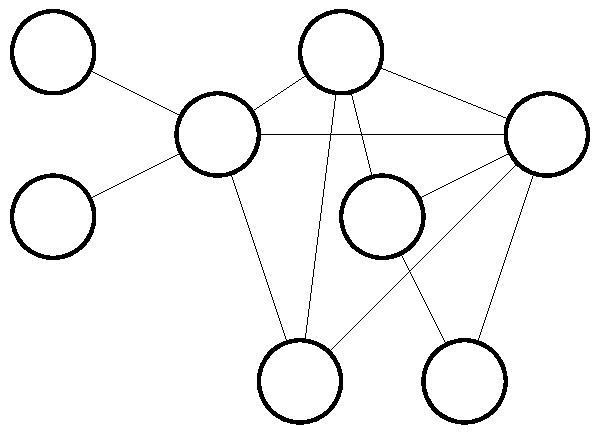
\includegraphics[scale=0.6]{images/4CLIQUE}	
	\end{center}
\end{frame}
\subsection{Aufgabe B9 A2}
\begin{frame}
	\frametitle{Aufgabe B9 A2}
	Gehen Sie bei dieser Aufgabe durchweg von der Annahme $\mathcal{P} \neq \mathcal{NP}$
	aus.
	\only<1>{
	\begin{tabbing}
	\textbf{Problem:} 4-COLOR\\
	\textit{Gegeben:} \= Ein ungerichteter Graph $G = (V,E)$\\
	\textit{Gesucht:} \> Gibt es eine F"arbung der Knoten $V$, sodass je zwei durch eine\\
	\> Kante aus $E$ miteinander verbundene Knoten unterschiedlich\\
	\> gef"arbt sind, wenn nur vier unterschiedliche Farben zur\\
	\> Verf"ugung stehen?
	\end{tabbing}
	Zeigen Sie, dass 4-COLOR $\mathcal{NP}$-vollst"andig ist!\\
	\underline{Hinweis:} Es kann hilfreich sein, wenn Sie die $\mathcal{NP}$-
	Vollst"andigkeit des Dreif"arbbarkeitsproblems 3-COLOR verwenden.
	}
	\only<2>{
	\\Es ist bekannt, dass sowohl das Erf"ullbarkeitsproblem der Aussagenlogik SAT als
	auch 3-SAT, das	Erf"ullbarkeitsproblem mit Beschr"ankung auf Klauseln mit nur 3
	Literalen, $\mathcal{NP}$-vollst"andig sind.\\
	Das Problem 3-CLIQUE ist wie folgt definiert:
	\begin{tabbing}
	\textbf{Problem:} 3-CLIQUE\\
	\textit{Gegeben:} \= Ein ungerichteter Graph $G = (V,E)$\\
	\textit{Gesucht:} \> Gibt es eine Clique (vollst"andig verbundener Teilgraph)\\
	\> der Gr"o"se $3$ in $G$?
	\end{tabbing}
	Zeigen Sie, dass 3-CLIQUE \textbf{nicht} $\mathcal{NP}$-vollst"andig ist!
	}
\end{frame}

\section{NP-Probleme}
\subsection{Partition}
\begin{frame}
	\frametitle{PARTITION}
	\begin{block}{Kurzdefinition}
	Teile eine Menge natürlicher Zahlen in zwei Teilmengen, sodass die Summen der Elemente der Teilmengen gleichgroß sind.
	\end{block}
	\begin{block}{Formal}
	Gegeben: Natürliche Zahlen $a_1,...,a_n \in \mathbb{N} \; (n \in 	\mathbb{N})$\\
	Gesucht: Gibt es eine Teilmenge $J \subseteq \{1,...,n\}$ mit\\
	\[\sum\limits_{1 \leq i \leq n, i \in J}a_i \; = \;
	\sum\limits_{1 \leq i \leq n, i \notin J}a_i \text{?}\]
	\end{block}
\end{frame}
\begin{frame}
	\frametitle{Beispiele}
	Welche dieser Mengen ist partitionierbar?
	\[\{16,8,4,3,1,1,1\}\]\\
	\[\{7,4,8,2,12,8,9,3,6\}\]\\
	\[\{5,8,9,2,6,4\}\]
\end{frame}

\subsection{Bin Packing}
\begin{frame}
	\frametitle{BIN PACKING}
	\begin{block}{Kurzdefinition}
	Teile eine Menge von Objekten mit Gewichten auf eine Menge von Behältern mit Maximallast, sodass jedes Objekt in einem Behälter ist und kein Behälter überladen ist.
	\end{block}
	\begin{block}{Formal}
	Gegeben: Eine Beh"altergr"o"se $b \in \mathbb{N}$, die Anzahl der
	Beh"alter $k \in \mathbb{N}$\\
	und Objekte $a_1,...,a_n \; (n \in \mathbb{N})$ mit\\
	$a_i \in \mathbb{N}, a_i \leq b$ f"ur alle $i \in \{1,...,n\}$\\~\\
	Gesucht: K"onnen die $n$ Objekte so auf die $k$ Beh"alter verteilt
	werden,\\
	dass kein Beh"alter "uberbeladen ist?\\
	\end{block}
\end{frame}
\begin{frame}
	\frametitle{Beispiel}
	Seien die Gewichte der Objekte $\{3, 1, 4, 5, 1, 1\}$~\\
	und es existieren 3 Behälter mit Maximalgröße 5~\\~\\
	Gibt es eine Verteilung ohne Überlastung?~\\~\\~\\~\\~\\~\\
	Seien die Gewichte der Objekte $\{5, 4, 3, 3\}$~\\
	und es existieren 3 Behälter mit Maximalgröße 5~\\~\\
	Gibt es eine Verteilung ohne Überlastung?
\end{frame}


\subsection{Aufgabe B9 A1}
\begin{frame}
	\frametitle{Aufgabe B9 A1}
	Gegeben sind die folgenden Probleme:
	\begin{tabbing}
	PARTITION:\\
	\textit{Gegeben:} \= Nat"urliche Zahlen $a_1,...,a_n \in \mathbb{N} \; (n \in
	\mathbb{N})$\\
	\textit{Gesucht:} \> Gibt es eine Teilmenge $J \subseteq \{1,...,n\}$ mit\\
	\> $\sum\limits_{1 \leq i \leq n, i \in J}a_i \; = \;
	\sum\limits_{1 \leq i \leq n, i \notin J}a_i$?\\[8pt]
	BIN PACKING:\\
	\textit{Gegeben:} \> Eine Beh"altergr"o"se $b \in \mathbb{N}$, die Anzahl der
	Beh"alter $k \in \mathbb{N}$\\
	\> und Objekte $a_1,...,a_n \; (n \in \mathbb{N})$ mit\\
	\> $a_i \in \mathbb{N}, a_i \leq b$ f"ur alle $i \in \{1,...,n\}$\\
	\textit{Gesucht:} \> K"onnen die $n$ Objekte so auf die $k$ Beh"alter verteilt
	werden,\\
	\> dass kein Beh"alter "uberbeladen ist?\\
	\end{tabbing}
	\only<1>{
	Zeigen Sie, dass BIN PACKING $\mathcal{NP}$-hart ist, wobei PARTITION als
	$\mathcal{NP}$-vollst"andig vorausgesetzt werden darf!
	}	
	\only<2>{Gegeben seien die Objekte der PARTITION-Probleminstanz
	$(a_1,a_2,a_3,a_4,a_5,a_6) = (1,1,2,3,4,5)$. Zeigen	oder widerlegen Sie, ob das transformierte und das urspr"ungliche Problem eine
	L"osung besitzen!
	}
\end{frame}

\section{Schluss}
\subsection{Schluss}
\begin{frame}
\frametitle{Bis zum nächsten Mal!}
\begin{center}
	%TODO Comic ändern
	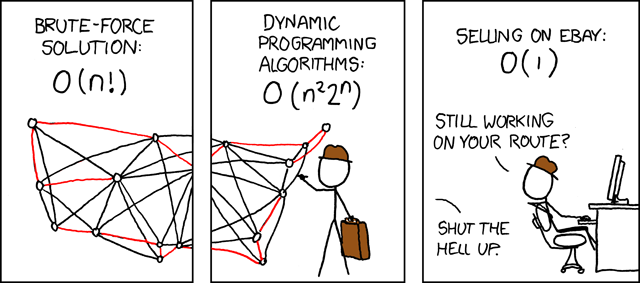
\includegraphics[width= \textwidth]{images/399_traveling_salesman}
\end{center}
\end{frame}

\frame{
  \frametitle{Lizenzen}
  \center
  
\includegraphics[width=2em]{images/by}
  
\includegraphics[width=2em]{images/cc}
  
\includegraphics[width=2em]{images/sa}
  \\
  {\tiny

Dieses Werk ist unter einem ``Creative Commons Namensnennung-Weitergabe unter gleichen Bedingungen 3.0 Deutschland``-Lizenzvertrag lizenziert. Um eine Kopie der Lizenz zu erhalten, gehen Sie bitte zu \href{http://creativecommons.org/licenses/by-sa/3.0/de/}{http://creativecommons.org/licenses/by-sa/3.0/de/} oder schreiben Sie an Creative Commons, 171 Second Street, Suite 300, San Francisco, California 94105, USA.\\
  \vspace{1cm}
  Davon ausgenommen sind das Titelbild, welches aus der März-April 2002 Ausgabe von American Scientist erschienen ist und ohne Erlaubnis verwendet wird, sowie das KIT Beamer Theme. Hierfür gelten die Bestimmungen der jeweiligen Urheber.
  \vspace{1cm}
  \\ 
  }
  %Habe hier die Reihenfolge etwas umgestellt, weil die Formatierung bei mir komisch aussah. 
  %Wenn es bei dir anders ist, kannst du es auch wieder zurückändern, dann haben wir unterschiedliche Kompilieroptionen
}

\end{document}